\documentclass[upright, contnum]{umemoria}

\depto{DEPARTAMENTO DE CIENCIAS DE LA COMPUTACIÓN}
\author{FELIPE ANIBAL RICARDO ESPINOZA CASTILLO}
\title{DISEÑO Y DESARROLLO DE UNA HERRAMIENTA DE REPRESENTACIÓN Y VISUALIZACIÓN DE REDES SOCIALES CON CAPACIDADES DISTRIBUIDAS}
\auspicio{}
\date{JULIO 2013}
\guia{CLAUDIO GUTIÉRREZ GALLARDO}
\carrera{TÍTULO DE INGENIERO CIVIL EN COMPUTACIÓN}
\comision{GONZALO NAVARRO BADINO}{LUIS MATEU BRULE}{\ }

\setcounter{secnumdepth}{4}
\setcounter{tocdepth}{4}
\usepackage{float}

\begin{document}
  \frontmatter
  \maketitle
  \begin{abstract}
  \begin{verbatim}
                                     RESUMEN DE LA MEMORIA
                                     PARA OPTAR AL TÍTULO DE:
                                     INGENIERO CIVIL EN COMPUTACIÓN
                                     POR: FELIPE ANÍBAL RICARDO ESPINOZA CASTILLO
                                     PROFESOR GUÍA: CLAUDIO GUTIÉRREZ GALLARDO
                                     FECHA: 12/07/2013
  \end{verbatim}

  \begin{center}
      \textbf{DISEÑO Y DESARROLLO DE UNA HERRAMIENTA DE REPRESENTACIÓN Y VISUALIZACIÓN DE REDES SOCIALES CON CAPACIDADES DISTRIBUIDAS}
  \end{center}
  
  % CONSIDERACIONES
  
  % Escrito en pasado
  % Una página que resume todo
  %   - Motivación
  %   - Problema
  %   - Solución desarrollada
  %   - Resultados obtenidos
  % Muy buena ortografía y redacción
  
  % - motivación (por qué?)
  % lo que veo en littlesis y la información al pueblo
  % herramienta de apoyo a investigadores
  
  % - problema (qué quiero resolver?)
  % entregar un sistema a los usuarios para que ellos puedan fácilmente modelar la información de redes sociales
  % modelo flexible y completo para estructuras de redes sociales
  
  % - solución desarrollada (qué cosa?)
  % aplicación web del lado del cliente con un servidor
  % uso de la experiencia de Manuel Bahamonde
  % uso de la experiencia y el modelod e Mauro
  
  % - resultados obtenidos (qué gané?)
  % Una aplicación cuyo ambiente puede ser fácilmente replicable
  % Permite la colaboración entre usuarios
  % Una aplicación de modelamiento de redes sociales genéricas
  
  Hoy existen diversas bases de datos centralizadas de relaciones de \emph{quién conoce a quién}, como LittleSis y Poderopedia, que contienen información de posibles conflictos de intereses entre las personas poderosas de un país.
  Ellas son de mucha  utilidad como medios de entrega de información a las personas. Ellas presentan un modelo de red social que puede ser replicado en otras áreas del conocimiento.\\
  
   Los investigadores y trabajadores sociales que se enfrentan con este tipo de estructuras sociales requieren aplicaciones que les faciliten su creación y manejo. Con el objetivo de apoyar el trabajo de estas personas, que no necesariamente tienen conocimientos avanzados de computación, en esta memoria se abordó la creación de una herramienta que le permitiera a sus usuarios crear y manejar información de las estructuras sociales en forma de redes en los contextos que los ellos estimen conveniente.\\
  
  Este trabajo partió de la experiencia de una memoria similar realizada anteriormente por el ex alumno del departamento Manuel Bahamonde. En este trabajo se mejoró su propuesta inicial, aplicando su experiencia y usando el modelo mejorado propuesto por Mauro San Martín en su tesis de doctorado.\\
  
  A partir de lo anterior, se creó una aplicación web que le permite al usuario realizar las tareas señaladas, con una interfaz amigable y usando las últimas tecnologías en lo que a desarrollo web se refiere. Esta aplicación  además permite la interacción entre los usuarios de la aplicación ya que les provee herramientas para combinar la información que producen entre ellos.\\
  
  Este trabajo presentó una gran gama de desafíos. Los cuales pasan por la de visualización manipulable de grafos, manejo de eventos, la implementación del modelo de redes sociales, entre otros. Se discute como se logró el objetivo propuesto y se sortearon estos desafíos. Adicionalmente, se logró un primer acercamiento a la integración con tecnologías de la web semántica, debido a que la información producida puede ser importada y exportada en formato RDF. Finalmente se indican los principales focos de mejora y avance de este proyecto.

\end{abstract}
  \begin{dedicatoria}
  A María Cristina, Andrés, Jorge y Simón.
\end{dedicatoria}
  \begin{thanks}
  Tengo mucho que agradecer y a muchas personas, quienes han estado junto a mí a lo largo de toda esta etapa del proceso de aprendizaje que concluye con este trabajo de memoria. Estas personas han contribuido de alguna u otra forma en los resultados obtenidos hoy, por lo tanto es una buena instancia para agradecer por ello.
  
  En primer lugar, quiero agradecer a mi profesor guía Claudio Gutiérrez con el cual mantuve una relación de trabajo fructífera y amena, desde la idea inicial de este trabajo hasta su resultado final, siendo un apoyo fundamental para el cumplimiento de objetivos de esta, especialmente en periodos de confusión.
  
  Quiero agradecer también a las personas con las que adquirí experiencia laboral y fueron amigos desde temprana edad. Estas personas me enseñaron mucho de cómo funciona la industria del software, aspectos técnicos, de negocio, entre otros. Estas personas son: Daniel Pizarro, Hernán Sánchez, Álvaro Faúndez de \emph{Firenxis}. Rolando Abarca, Felipe Bascuñán y Juan Francisco Rodríguez de \emph{Games for Food}. David Assael, David Basulto y Gustavo García de \emph{ArchDaily}. Personas quienes me entregaron responsabilidad, confianza y conocimiento para desenvolverme como profesional desde un inicio.
  
  También tengo que agradecer a los amigos que han estado conmigo, me han entregado su cariño y me han enseñado muchas cosas útiles en la vida. Ellos son: Camilo López, Carlota González, Juan Muñoz, Paola Veliz, César Nuñez, Andrés Rebolledo, Laura Barahona, Karla Elorza, Laura Lagos, Diana Vásquez, Melanie y Melissa Villavicencio, entre muchos otros más.
  
  Además quiero mencionar a personas muy especiales que me enseñaron muchas cosas y acompañaron en las etapas que enfrenté a lo largo de los años: Giuliana Lunecke y Fabiola Quezada. Además una mención especial a Soledad Palma, quien estuvo siempre a mi lado en el desarrollo de esta memoria.
  
  Finalmente mis agradecimientos más grandes a mi familia: María Cristina, Andrés Godoy, Jorge Jesús Orellana y Simón Orellana. Quienes siempre me han entregado amor, comprensión y apoyo incondicional. De no ser por ellos no hubiera logrado las cosas que estoy logrando hoy en día.
  
  A todas estas personas, mis más sinceros agradecimientos, por todo.
\end{thanks}
  \tableofcontents
  \listoftables
  \listoffigures
  \mainmatter
  
  %=== BEGIN cuerpo de la memoria
    \begin{intro}
  % -- Contexto y littlesis --
  Existe una red social llamada \textbf{LittleSis}\cite{littlesis} que consiste en una base de datos de relaciones de \emph{quien conoce a quien} entre gente política, económica y socialmente poderosa en el mundo de las organizaciones en Estados Unidos cuyo fin es entregar el poder de la información al pueblo.\\

  El origen del nombre de \emph{LittleSis} se relaciona con el personaje \emph{Big Brother} de la novela de George Orwell llamada \emph{Nineteen Eighty-Four}. Este personaje consiste en un dictador que maneja toda la información sobre la población. \emph{Big Brother} posteriormente fue un concepto con el cual se describió un ente poderoso.\\
 
  De esta forma, al grupo compuesto por las personas poderosas y políticos de un país se les atribuye esta imagen de \emph{Big Brother}, por su poder e influencia en un país. Esta es la motivación para bautizar con el nombre \emph{LittleSis}\emph{(Little Sister)}, en oposición a \emph{Big Brother}, a una aplicación cuyo fin es entregar poder de la información a toda la población en lugar de esta minoría poderosa.\\

  La idea detrás de \emph{LittleSis} tiene la capacidad de ser replicada en muchos países con el mismo fin, esto es, el de entregar poder al pueblo e informarle sobre los posibles conflictos de interés que las autoridades locales y/o nacionales puedan tener al lidiar con el ejercicio de su poder, lo que en el caso particular de Chile, existe una iniciativa llamada \textbf{Poderopedia}\cite{poderopedia} que busca ser una réplica de \emph{LittleSis} para Chile.\\

  En el caso de \textbf{Poderopedia}, uno de los líderes de ese proyecto es el ex alumno del DCC, Álvaro Graves, quienes tienen un \textbf{modelo RDF publicado en un repositorio en Github}\cite{podervocabulary}, tienen el sitio de Poderopedia funcionando, el cual al igual que LittleSis es un repositorio centralizado de información sobre la gente de poder político y económico de Chile, sus relaciones entre sí y su relación con organizaciones.

  % -- Deficiencias de littleSis --
  Con toda sus potencialidades, tanto \emph{LittleSis} como \emph{Poderopedia}, poseen un fin muy particular. En este sentido, sólo tienen la capacidad de cubrir la información sobre las personas muy importantes del mundo político, social y económico poderoso. Pero si una persona quisiera recolectar información sobre grupos de personas (por ejemplo la red social de la comunidad investigadora en computación dentro de latinoamérica) para formar una red social, estas plataformas no sirven. Tampoco estas herramientas permiten la creación de redes sociales privadas, que cumplan los objetivos que el usuario desee, pero al mismo tiempo permitirle interactuar con los datos de otras redes sociales pertenecientes a otras personas o comunidades.\\

  % -- En esta parte se propone el proyecto ---
  El objetivo de esta memoria es llenar ese vacío, diseñando y desarrollando una herramienta para representar redes sociales, y que tengan capacidades distribuidas, donde los usuarios que poseen sus redes sociales públicas o privadas, puedan unirlas y compartirlas a voluntad.\\

  Esta herramienta posee una gran gama de aplicaciones posibles, tanto para estudios de tipo sociológico, histórico, biológico, político, etc. Un caso de ejemplo reciente es el caso de las redes de autoridades e intereses posibles dentro del ambiente educacional chileno, lo que puede dar una visión más informada sobre el entramado de intereses detrás de los problemas denunciados por el conflicto estudiantil que se vive desde el año 2011.\\

  % -- Desafíos técnicos --
  % --- Basado en el modelo de Mauro
  % --- ??
  Para lograr desarrollar esta herramienta se deben sortear una serie de desafíos técnicos, que aunque pareciera una aplicación bastante intuitiva, hasta el momento no hemos encontrado una aplicación con estas características.\\

  Entre sus mayores desafíos está el de tener una aplicación de fácil instalación y uso amigable para los usuarios. Por otro lado, con lo que respecta al modelamiento de datos, debe basarse en algún estándar flexible de representación de redes sociales que permita la interoperabilidad. Esta memoria partirá de la base y la experiencia del recientemente titulado doctor en computación Mauro San Martín, cuya tesis de doctorado consistió en diseñar un modelo para el manejo de redes sociales, de esta forma, se aprovechará el conocimiento de su experiencia de investigación, aplicándolo a un trabajo práctico y útil para la investigación y estudio de varias disciplinas.\\

  También habrá que desarrollar el aspecto de la visualización de datos, la integración con otras herramientas enfocadas al análisis de redes sociales, el modelamiento y uso de la información de redes sociales.\\

  Dado que la estructura de redes sociales está fuertemente ligada a grafos, y se necesita un estándar aceptado (para el que existan herramientas de desarrollo disponibles), se ha optado por representarlo en el modelo \textbf{RDF}. Este estándar es además es una representación que permitirá todo tipo de usos incorporándose a tecnologías de la \textbf{Web Semántica}. Finalmente, además de los anteriores, hay desafíos de negocios que se vinculan con lo técnico, como hacer algunos casos de prueba de usabilidad para entregar una herramienta de valor a usuarios y contactar diversas personas que puedan estar interesadas en la herramienta.\\

  % -- Organización del documento --
  Este informe comprende toda la experiencia al realizar esta memoria, las motivaciones, soluciones propuestas y resultados obtenidos durante el periodo de la misma. En el capítulo~\ref{chap:descripcion_proyecto} se presentan los objetivos y alcances para este trabajo. En el capítulo~\ref{chap:marco_conceptual} se abordan los conceptos relacionados a redes sociales y de desarrollo que son útiles para entender el resto del informe. En el capítulo~\ref{chap:especificacion_problema} se aborda en mayor medida el contexto en el cual se desarrolla el problema y se extraen los puntos principales a resolver. Luego en el capítulo~\ref{chap:descripcion_solucion} se documenta la arquitectura conceptual y concreta de la aplicación desarrollada para solucionar lo planteado en todo sus detalles, en el capítulo~\ref{chap:funcionamiento_solucion} se expone como esta solución funciona y finalmente se discuten las conclusiones del trabajo y sus alternativas a futuro.\\
  
\end{intro}
    \chapter{Descripción del Proyecto}

\section{Objetivos} % (fold)
\label{sec:objetivos}
A continuación se presentan los objetivos para este trabajo de memoria.

\subsubsection{Objetivo General} % (fold)
\label{ssub:objetivo_general}

El objetivo de este trabajo consiste en crear una herramienta por la cual personas que estudian diversos tipos de redes
sociales como: sociólogos, periodistas, biólogos, etc; puedan representar, administrar y visualizar redes sociales
de mediana escala, contando además con la capacidad de combinar redes sociales con otros usuarios de la herramienta
para obtener redes sociales con información más completa ofreciendo esto como un servicio centralizado con la
capacidad de ser distribuido.

% subsubsection objetivo_general (end)

\subsubsection{Objetivos Específicos} % (fold)
\label{ssub:objetivos_específicos}

De lo escrito anteriormente en el objetivo general, se desprenden los siguientes objetivos intermedios:

  \begin{enumerate}
    \item Implementar un modelo de representación de redes sociales en RDF.
    \item Hacer una interfaz amigable de ingreso de datos: actores y relaciones.
    \item Desarrollar un sistema centralizado que administre la asignación de identificadores únicos a los actores que los usuarios agregan a sus redes sociales.
    \item Unir redes sociales, combinando la información y relaciones de actores en común.
    \item Visualización
      \begin{enumerate}
        \item De la estructura general de las redes sociales creadas.
        \item Específica de elementos de interés en esas redes sociales.
      \end{enumerate}
    \item Representar algunas redes con el modelo implementado anteriormente, que varíen en tamaño y en complejidad.
  \end{enumerate}

% subsubsection objetivos_específicos (end)
% section objetivos (end)

\section{Resultados Esperados} % (fold)
\label{sec:resultados_esperados}

Para llevar a cabo los objetivos expuestos en esta memoria, los resultados que se esperan consisten en: un sistema que permita el modelamiento de redes sociales en donde debe existir una aplicación que permita de manera cómoda crear estas redes sociales, complementar su información para posteriormente unir las redes de un usuario con otro en caso de que este lo quiera. Además de lo anterior, los datos generados por el sistema deben estar en un formato amigable para computadores, que faciliten la posterior interoperabilidad con otras aplicaciones y fuentes de conocimiento.

% section resultados_esperados (end)

\section{Alcances} % (fold)
\label{sec:alcances}
% Especificar algunas limitaciones al problema a resolver con el fin de que la memoria sea un paso más acotado en la
% solución final del problema:
% 
% * se resolverá el problema para redes sociales de menos de 100 actores **Tamaño pequeño, revisar este número**
% * no se considerará la posible temporalidad de la red social

Es importante mencionar, que con el objetivo de que el trabajo a realizar cumpla con las limitaciones de tiempo correspondientes a una memoria de ingeniería, el problema de la creación y manipulación de redes sociales por personas se acota en los siguientes aspectos:

\begin{itemize}
  \item El tamaño de redes sociales, se considerará pequeño con un número de alrededor 100 actores por red social, debido a que las redes serán principalmente creadas de forma manual, por tanto debe manejar un número que sea posible de alcanzar por los usuarios de la aplicación, de esta forma, ahorrando problemáticas asociadas con la escalabilidad de la aplicación para redes sociales más grandes.
  \item Dependiendo de las aplicaciones para las cuales se use el modelamiento de redes sociales, puede requerirse ver los cambios temporales que sufren estas, para analizar la estructura de una red social y su evolución en el tiempo. Dicho problema no será abordado en esta memoria.
\end{itemize}
% section alcances (end)
    \chapter{Marco Conceptual}

En este capítulo se describen los conceptos necesarios para que el lector se pueda familiarizar con mayor facilidad con los conceptos usados en el resto del informe, describiendo lo que se entiende por los conceptos usados en términos de redes sociales y conceptos asociados al desarrollo de la solución.\\

En caso de así preferirlo, el lector puede saltar las secciones que estime convenientes dentro de este capítulo, en caso de dominar los conceptos y usar este capítulo como referencia en caso de necesitarlo.

\section{Conceptos de Redes Sociales} % (fold)
\label{sec:conceptos_de_redes_sociales}


A continuación se expondrán los conceptos fundamentales que se usarán en la memoria en relación a redes sociales. Estos conceptos fueron extraídos desde la tesis de doctorado del alumno del DCC, Mauro San Martín\cite{tesismauro}, debido a que representan lo necesario para el entendimiento de este trabajo, por lo tanto su reusó e inclusión en el informe para que el lector no necesite revisar la memoria de Mauro para poder ver estos conceptos.

Para construir la definición formal de redes sociales, es necesario definir algunos conceptos claves previamente, siguiendo las definiciones clásicas de este dominio\cite{sna}.

\subsection{Actor} % (fold)
\label{sub:actor}
Un actor es una entidad social, la cual está bajo estudio junto con sus interacciones sociales. En estricto rigor, los actores pueden ser definidos como individuos, corporaciones o unidades sociales colectivas. Ejemplos de actores son gente en un grupo, departamentos en una empresa o agencias de servicio público en una cuidad. El uso del término actor no significa que estas entidades necesariamente tienen la habilidad de actuar. Más allá, la mayoría de las aplicaciones en redes sociales se enfocan en colecciones de actores que son de un mismo tipo (por ejemplo, gente en un grupo de trabajo). A veces, sin embargo, la investigación necesita mirar a actores de diversos niveles o tipos conceptuales, o desde diversos conjuntos. Los datos pueden incluir atributos no relacionales asociados a los diferentes actores.
% subsection actor (end)

\subsection{Uniones Relacionales} % (fold)
\label{sub:uniones_relacionales}
Los actores están conectados hacia otros por uniones sociales. El rango y tipo de estas uniones puede ser muy grande. La característica principal de una unión es que establece una conexión entre un par de actores. Algunos de los ejemplos más comunes de uniones empleadas en el análisis de redes sociales son:

  \begin{itemize}
    \item La evaluación de una persona por otra, ej: amistad declarada, gusto o respeto.
    \item Transferencia de recursos materiales, ej: transacciones de negocios, prestar o pedir prestado.
    \item Asociación o afiliación, ej: atender conjuntamente a un evento social, o pertenecer al mismo club social.
  \end{itemize}
% subsection uniones_relacionales (end)

\subsection{Relaciones} % (fold)
\label{sub:relaciones}
El conjunto de uniones entre un tipo específico de miembros de un grupo se llama una relación. Por ejemplo, el conjunto de las amistades entre pares de niños en un salón de clases, o el conjunto de uniones diplomáticas entre pares de naciones en el mundo, son uniones que definen relaciones. Para cualquier grupo de actores, podemos encontrar diversas relaciones; por ejemplo, además de las relaciones diplomáticas entre países, podemos encontrar la existencia de comercio en un determinado año. Las relaciones (o uniones específicas) pueden tener atributos que las describen. Por ejemplo en el caso del comercio, su cantidad de transacciones total puede haber sido guardado.
% subsection relaciones (end)

Con lo expuesto anteriormente, finalmente podemos definir una red social.

\subsection{Red Social} % (fold)
\label{sub:red_social}
Una red social consiste en uno o muchos conjuntos finitos de actores, junto con las relaciones definidas entre ellos. La presencia de información relacional es una característica crítica de las redes sociales. Una red social es un caso particular de red, de esta manera su estructura puede ser formalizada como un grafo.

% TODO: cita aquí
En adición al uso de conceptos relacionales, Wasserman y Faust\cite{sna} se deben tener en cuenta las siguientes consideraciones:

  \begin{itemize}
    \item Actores y sus acciones son vistos como interdependientes, más que independientes, unidades autónomas.
    \item Uniones relacionales (conexiones) entre actores son canales de transferencia o "flujo" de recursos (material o no material).
    \item Modelos de red enfocados en individuos muestran el ambiente estructural de la red, además de proveer la capacidad de definir limitaciones en nivel individual.
    \item Los modelos de red conceptualizan estructura (social, económica, política, entre otras) como patrones generales de relaciones entre actores.
  \end{itemize}
% subsection red_social (end)


% ### 2.1 Conceptos de Redes Sociales
% 
% * explicación de que se van a reusar (copiar-pegar casi) los conceptos de redes sociales de la tesis de mauro
% 
% #### 2.1.1. Definiciones
% 
% * red social
% * nodo {NO}
% * actor
% * atributo {NO}
% * relación
% * familia {NO}
% * rol {NO}

% {NO} es pq estos conceptos son más específicos al modelo de mauro, pues se entienden mejor con el modelo

\section{Conceptos de Desarrollo} % (fold)
\label{sec:conceptos_de_desarrollo}

A continuación se explican los términos en lo que a desarrollo que se refiere que tienen relación con el trabajo realizado en esta memoria.

\subsection{Desarrollo Web} % (fold)
\label{sub:desarrollo_web}

% * que es el desarrollo web
% * arquitectura de cliente servidor
% * que componentes típicos se encuentran en el desarrollo web
%   * servidor
%   * browser
%     * web
%     * movil
%   * servidor de bases de datos
%   * servidor de acceso a aplicaciones

El desarrollo web se denomina al desarrollo de software cuyo fin es la creación de aplicaciones que se ejecuten en computadores que puedan ser accesados vía la \emph{world-wide web}. Este estilo de desarrollo conlleva a que una aplicación que pueda estar ejecutándose en un servidor pueda entregar resultados a clientes provenientes de cualquier parte del mundo, usando una gran diversidad de dispositivos, plataformas de software, etc. Las cuales son frecuentemente accesadas por personas vía un navegador web.\\

Esta propiedad de multiplataforma de las aplicaciones desarrolladas para la web, junto con propiedades de accesibilidad desde diversos medios a las aplicaciones, ha hecho que el desarrollo web sea un enfoque de desarrollo ampliamente usado en la industria en los últimos 10 años.\\

En términos generales el desarrollo web posee una arquitectura clásica de cliente/servidor, en donde una aplicación corriendo en un servidor proporciona resultados y ejecuta instrucciones proveniente de clientes, que pueden ir desde un navegador web de p.c. o dispositivo móvil, o servir de API, \emph{Application Programming Interface}, para otras aplicaciones. A continuación se adjunta un diagrama que muestra los principales componentes cuando se habla de desarrollo web.\\

A modo de ejemplo de componentes en el desarrollo web de una aplicación que posee un servidor de ejecución de la aplicación, con un servidor de base de datos, que es accesada vía teléfono, tablet o computador por medio de un navegador web o de una interfaz API que use otra aplicación, por la cual se acceden sus datos en formato de documentos HTML (junto con sus estilos en CSS y manejo de eventos en JavaScript) o documentos en formato JSON, RDF, XML entre otros.\\

Dentro del desarrollo web, también se encuentran subcategorías que son expuestas a continuación.

\subsubsection{Desarrollo Front-End} % (fold)
\label{ssub:desarrollo_front_end}
% * es el desarrollo que compone todos los aspectos de un sistema con los cuales interactúa un cliente, como el cliente
% la arquitectura de cliente-servidor

Es el desarrollo orientado a todos los componentes con los cuales interactúa un usuario de la aplicación, enfocado en la interfaz y sus componentes gráficos, además de la experiencia usuario, la usabilidad de la aplicación, etc. Es el desarrollo del cliente que el usuario usa para acceder al core de la aplicación.\\

En términos de tecnologías, se asocia el desarrollo front-end al uso de tecnologías como: HTML, CSS, Javascript, entre otras.
% subsubsection desarrollo_front_end (end)

\subsubsection{Desarrollo Back-End} % (fold)
\label{ssub:desarrollo_back_end}

% * es desarrollo de software de la aplicación que guarda y procesa los datos del usuario

Es el desarrollo de la aplicación que almacena y posee la lógica común a todos los clientes de la aplicación, en donde el código de este tipo de desarrollo es que se ejecuta en el servidor. Además generalmente en el desarrollo back-end se incluye todo lo relacionado a persistencia de datos generados a través del uso de la aplicación.

% subsubsection desarrollo_back_end (end) 
% subsection desarrollo_web (end)

\subsection{Modelo MVC} % (fold)
\label{sub:modelo_mvc}
El modelo MVC (Modelo, Vista, Controlador)\cite{mvc}, consiste en un modelo para separar la lógica de una aplicación agrupándola en clases u otras unidades modulares, de acuerdo con la responsabilidad que estos módulos cumplan dentro de un sistema. A modo de ejemplo, a fin de ilustrar este concepto, se puede dar un caso de una aplicación que registre compras en un sistema de tienda online, un ejemplo de los módulos asociados a compras en MVC puede ser el siguiente:

\begin{figure}[!h]
  \centering
  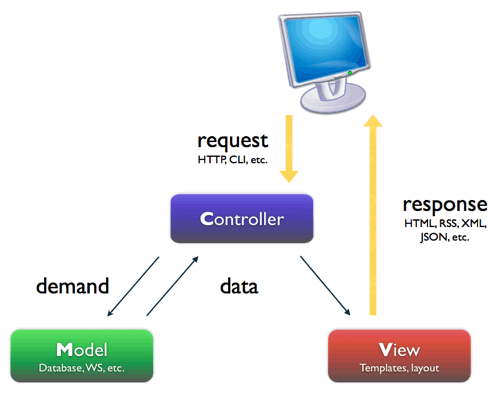
\includegraphics[scale=.5]{images/mvc.png}
  \caption{Modelo MVC}
  \label{modelomvc}
\end{figure}

\begin{itemize}
  \item \textbf{Modelo}: el modelo corresponde a una clase \texttt{Compra} que contiene toda la lógica de negocio asociada a las compras, que además se asocia directamente a como se almacena una compra en la base de datos.
  \item \textbf{Vista}: un ejemplo de vista para una compra, puede ser una interfaz \texttt{HTML} en la cual el cliente efectúe operaciones sobre la compra, por ejemplo agregar productos, cabe destacar que la vista no ejecuta las acciones, sólo se encarga de recibirlas y enviarlas al último componente del modelo MVC, el controlador.
  \item \textbf{Controlador}: de acuerdo a lo recién expresado, el controlador es el encargado de coordinar uno o más modelos para ejecutar las acciones capturadas en la vista. En el caso de la compra, el controlador es quien efectivamente procesaría el pago de la misma.
\end{itemize}
% subsection modelo_mvc (end)

\subsection{Frameworks de Desarrollo} % (fold)
\label{sub:frameworks_de_desarollo}
Un framework de desarrollo define un marco en el cual desarrollar una aplicación, el cual provee una gran cantidad de funcionalidad común lista de manera de no desarrollar un proyecto desde cero, pero además de sólo funcionalidad, provee de una estructura lógica con la cual se escribe el código, que está influida por muchas otras personas que han usado el framework en aplicaciones reales.

\subsubsection{Frameworks Server Side} % (fold)
\label{ssub:frameworks_server_side}
Dentro de los frameworks de desarrollo web existe una categoría llamada \emph{Sever Side}, la cual consiste en que el código de la aplicación corre desde un servidor en internet, lo que permite que si la computación es común para muchos clientes, los resultados de esa computación pueden ser usados múltiples veces.\\

Ejemplos actuales de esta categoría de frameworks son: \texttt{Ruby on Rails}\cite{rails}, \texttt{Sinatra}\cite{sinatra} que utilizan el lenguaje \texttt{Ruby}; \texttt{Django}\cite{django}, \texttt{Pylons}\cite{pylons} para \texttt{Python}; \texttt{Spring}\cite{spring} para \texttt{Java} y \texttt{CakePHP}\cite{cake} para PHP entre otros.
% subsubsection frameworks_server_side (end)

\subsubsection{Frameworks Client Side} % (fold)
\label{ssub:frameworks_client_side}
En el último tiempo, surgió una nueva categoría de frameworks de desarrollo web llamada \emph{Client Side}, en la cual el código de la aplicación se ejecuta en el computador del usuario de la aplicación, ahorrando recursos necesarios en un servidor, además de ahorrar el tiempo de latencia entre el cómputo de una respuesta y su transmisión al equipo del usuario.\\

Comúnmente estos frameworks son escritos para ser usados con el lenguaje \texttt{Javascript}, pues posee la propiedad que todos los navegadores web implementan un motor de \texttt{Javascript} y por lo tanto el usuario no necesita instalar nada más. Ejemplos de frameworks client side son: \texttt{AngularJS}\cite{angular}, \texttt{EmberJS}\cite{ember}, \texttt{Meteor}\cite{meteor} y alternativamente \texttt{BackboneJS}\cite{backbone} que es una librería más que un framework.
% subsubsection frameworks_client_side (end)

% subsection frameworks_de_desarollo (end)

% #### 2.2.5. HTML5
% 
% * a que se llama HTML5
% * que entrega a diferencia de las versiones anteriores
% 
% ##### 2.2.5.1 SVG, Gráficos Vectoriales en la Web
% 
% * que son y de que sirven estos gráficos (redimensión, formato común xml, etc)
\subsection{HTML5} % (fold)
\label{sub:html5}

\emph{Html5}\cite{html5} es el nuevo estándar para \emph{HTML}, Hyper-Text Markup Language, definido por la WC3\cite{w3c} y Web Hypertext Application Technology Group (WHATWG), es un trabajo en progreso, sin embargo desde hace tiempo los principales navegadores soportan muchas de los nuevos elementos de HTML y sus APIs.\\

Algunas de los nuevas características más interesantes en HTML5 son: el tag \texttt{<canvas>} para dibujo en 2D, los tags \texttt{<video>} y \texttt{<audio>} para reproducción multimedia, soporte para almacenamiento local en el browser, algunos elementos específicos para el contenido como \texttt{<article>}, \texttt{<footer>}, \texttt{<header>}, \texttt{<nav>} y \texttt{<section>}; nuevos controles para formularios como para fecha, hora, email, url y búsqueda. Además de esto, soporte para SVG dentro de los sitios, característica especialmente importante para esta memoria.

\subsubsection{SVG, gráficos vectoriales en la web} % (fold)
\label{ssub:svg_graficos_vectoriales_en_la_web}

SVG, en inglés se refiere a gráficos vectoriales escalables, los cuales pueden ser usados directamente en documentos HTML5, de manera de crear gráficos complejos en un formato de tipo XML. La diferencia de este tipo de gráficos con respecto a imágenes por ejemplo, es que los gráficos SVG no pierden calidad si son redimensionados o se ven sus detalles por medio de una funcionalidad de lupa. Estos elementos son altamente animables y corresponde a una recomendación por parte de la W3C\cite{w3c}.

% subsubsection svg_gráficos_vectoriales_en_la_web (end)

% subsection html5 (end)


% section conceptos_de_desarrollo (end)
    \chapter{Especificación del Problema}
\label{chap:especificacion_problema}

\section{Antecedentes y soluciones existentes} % (fold)
\label{sec:antecedentes_y_soluciones_existentes}

A continuación se presentan algunas de las soluciones existentes que apuntan a resolver problemas similares al de esta memoria.

\subsection{LittleSis y Poderopedia} % (fold)
\label{sub:littlesis_y_poderopedia}

% * que es littlesis
% * screenshot de littlesis
% * por que no cumplo el objetivo de la memoria con littlesis
\textbf{LittleSis}, pequeña hermana en oposición al gran hermano (Big Brother), es una plataforma estadounidense que contiene una base de datos libre de relaciones de \emph{quien conoce a quien} en el mundo de las grandes empresas y políticas de ese país. Todo esto con el fin de entregar información a la gente sobre qué posibles conflictos de intereses pueden tener los políticos que toman las decisiones en el país.

\begin{figure}[H]
  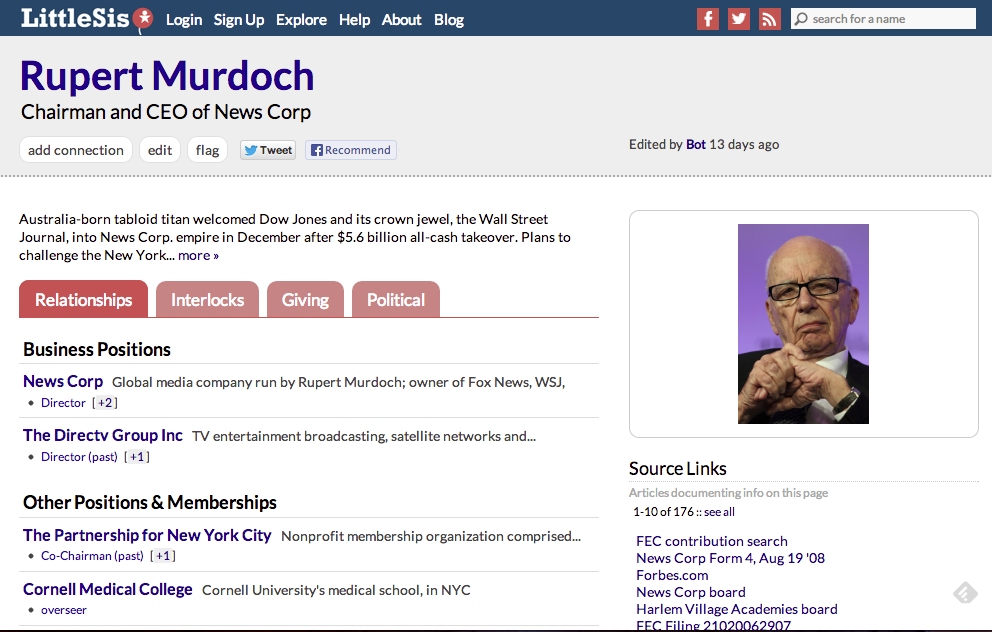
\includegraphics[width=1.0\textwidth]{images/littlesis.png}
  \caption[Interfaz de LittleSis, Rupert Murdoch]{\emph{Interfaz de LittleSis, Rupert Murdoch}. Un ejemplo de como littlesis almacena la información de las personas y el tipo de personas presentes en littleSis.}
  \label{ejemplo_littlesis}
\end{figure}

La idea detrás de LittleSis de entregar el poder de la información a la gente es muy buena desde su punto de vista de análisis de estructuras sociales económicas y políticas. Sin embargo, no cubre el problema que trata resolver esta memoria, debido a que si bien las personas pueden complementar esta información, esto se hace de una manera centralizada, además de que no se puede agregar información asociada a otro tipos de redes sociales, como por ejemplo: la red de panaderos de un país, ya que no está dentro del objetivo y alcance de LittleSis, sin mencionar que esta idea está enfocada en Estados Unidos.\\

\textbf{Poderopedia} es el clon chileno de LittleSis, una plataforma centralizada por la cual se expone información sobre las redes de poder e influencias en el ambiente económico, social y político chileno, en donde nuevamente el objetivo es enfocarse en las personas de los más altos cargos empresariales y políticos en Chile.\\

\begin{figure}[H]
  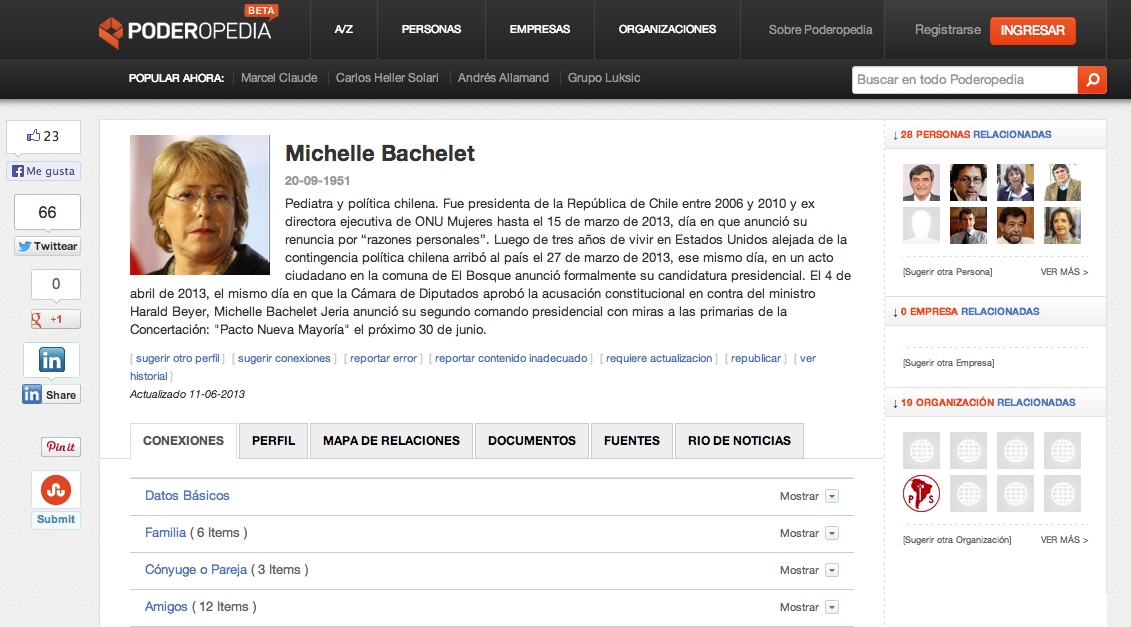
\includegraphics[width=1.0\textwidth]{images/poderopedia.png}
  \caption[Interfaz de Poderopedia, Michelle Bachelet]{\emph{Interfaz de Poderopedia, Michelle Bachelet}. Un ejemplo de como poderopedia almacena la información de las personas y el tipo de personas presentes en esta plataforma.}
  \label{ejemplo_poderopedia}
\end{figure}

\begin{figure}[H]
  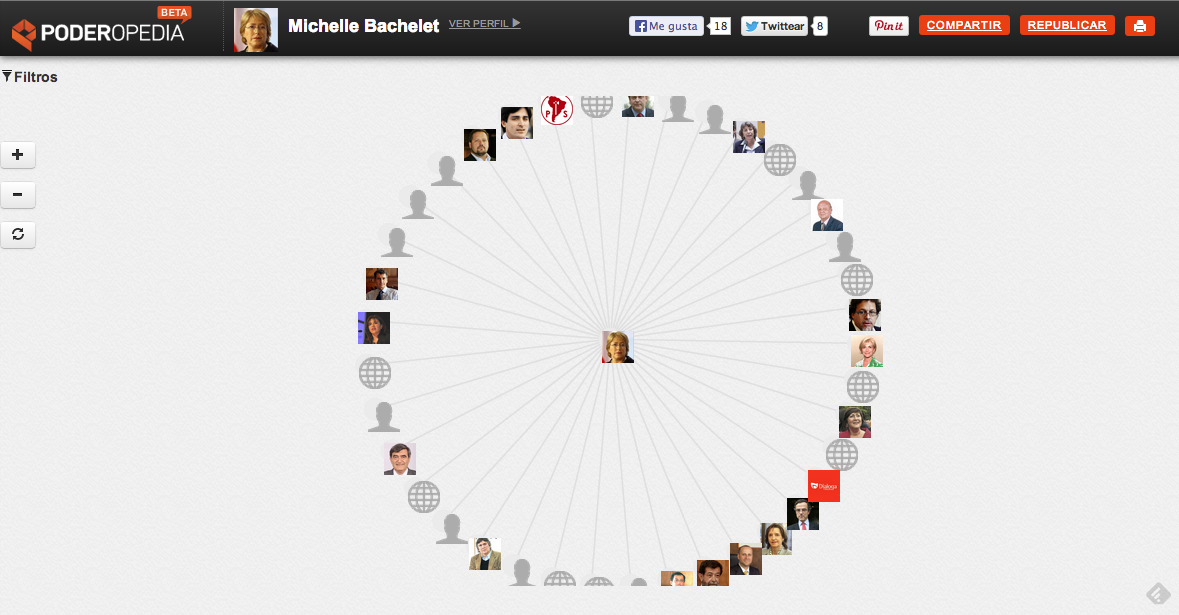
\includegraphics[width=1.0\textwidth]{images/grafo_poderopedia.png}
  \caption[Interfaz de Grafo de Poderopedia, Michelle Bachelet]{\emph{Interfaz de Grafo de Poderopedia, Michelle Bachelet}. Poderopedia tiene una opción de visualización de grafo al rededor de una persona.}
  \label{ejemplo_grafo_poderopedia}
\end{figure}

De la misma forma de LittleSis, las desventajas de Poderopedia en relación al problema que se desea resolver en esta memoria, van por el lado de que su foco es exclusivamente la gente con poder político y económico del país, que además es centralizada, que su visualización de grafo no entrega información real de las estructuras sociales y no es fácilmente manipulable.\\

Ambos LittleSis y Poderopedia son excelentes herramientas, pero su objetivo difiere de lo que se desea resolver en esta memoria, a pesar de que la idea básica es la misma, exponer información sobre estructuras sociales.

% subsection littlesis_y_poderopedia (end)

\subsection{Memoria Manuel Bahamonde} % (fold)
\label{sub:memoria_manuel_bahamonde}

Un intento de resolver este problema fue desarrollado por el alumno del DCC Manuel Bahamonde, quien hizo su trabajo de memoria titulado: \emph{Aplicación para la creación y administración de redes sociales} \cite{memoriamanuel} el año 2009, memoria también guiada por el profesor Claudio Gutiérrez. Entonces, se gestó la idea de este trabajo de memoria, como una forma de mejorar lo desarrollado anteriormente por Manuel, aprovechando los avances tecnológicos y experiencias con el modelamiento de redes sociales y la web semántica.\\

La aplicación desarrollada en Java por Manuel, permite al usuario descargar un ejecutable y usarlo tanto en Windows, Linux o Mac, la cual permite crear redes sociales en forma de grafo, creando actores y sus relaciones respectivas, asociándolos a familias y pudiendo exportar la información de las redes sociales en formato para la utilización del software de análsis de redes sociales, pajek\cite{pajek}.

\begin{figure}[H]
  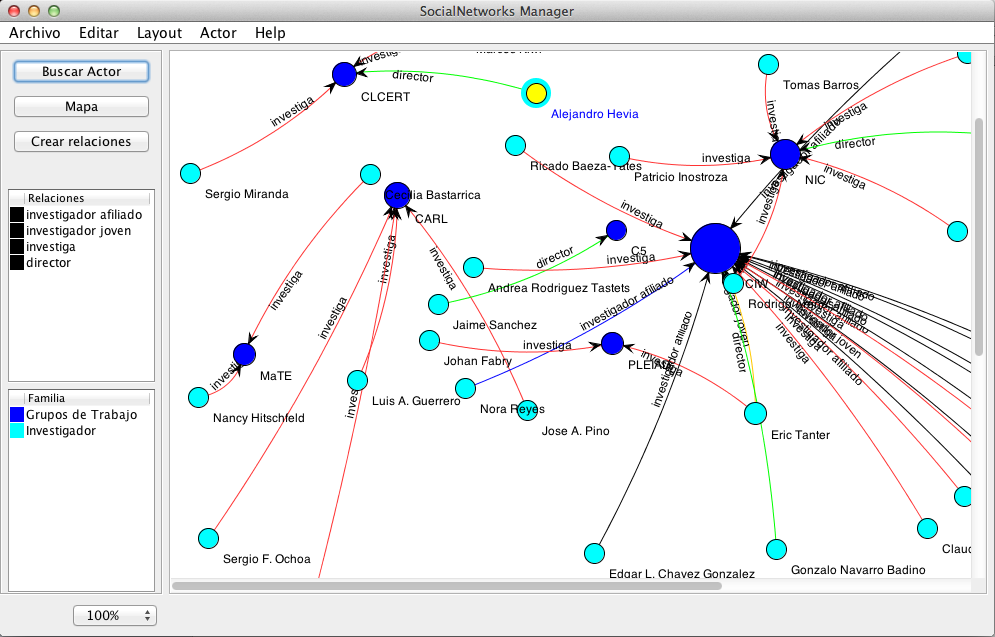
\includegraphics[width=1.0\textwidth]{images/memoria_manuel.png}
  \caption[Interfaz SocialNetworks Manager]{\emph{Interfaz SocialNetworks Manager}. La aplicación creada por el alumno Manuel Bahamonde con el objetivo de modelar redes sociales como aproximación incial al problema de esta memoria.}
  \label{memoria_manuel}
\end{figure}

El trabajo de Manuel ayudó como experiencia para acercarse más a una solución para el modelamiento de redes sociales y con el conocimiento actual del tema, es necesario hacer modificaciones a lo que hizo Manuel, resolviendo algunos problemas extras, como:

  \begin{enumerate}
    \item El formato de almacenamiento de las redes sociales, no permite una interoperabilidad con otras aplicaciones fuera de pajek\cite{pajek}, en especial con las tecnologías de la web semántica.
    \item Las relaciones entre actores sólo pueden ser 2 actores a la vez, no hay posibilidad de crear n-relaciones, o relaciones entre $n$ actores.
    \item Esta aplicación no permite complementar la información de una red social uniéndola con otra.
    \item No se puede agregar atributos a los actores y relaciones.
    \item Necesita que el usuario de la aplicación tenga instalado Java en su equipo.
    \item No se puede acceder a la información del usuario desde cualquier computador.
    \item La interfaz podría ser mejor en términos de usabilidad
  \end{enumerate}

% subsection memoria_manuel_bahamonde (end)

\subsection{Otras Alternativas} % (fold)
\label{sub:otras_alternativas}

% * que otras referencias de soluciones similares tengo?

Dentro de las otras opciones disponibles al tema de esta memoria, se tiene algunos softwares de creación y visualización de grafos, como por ejemplo yED\cite{yed} u OnmniGraffle\cite{omnigraffle}. Este tipo de soluciones sólo genera los grafos de forma visual, sin tener los datos estructurados de la red para poder ser analizados posteriormente por otra aplicación, además de que no ayudan con la creación efectiva de redes sociales, pues no poseen un esquema concreto de redes sociales por ser herramientas de visualización multipropósito.\\

Otras herramientas existentes de la rama de análisis de redes sociales son por ejemplo Gruff\cite{gruff} que es una herramienta de visualización de la base de datos AllegroGraph\cite{allegrograph}, la cual no posee las características que permiten crear redes sociales en forma estructurada, en base a un modelo estándar que se sepa que funciona, como el modelo SNM de Mauro San Martín\cite{tesismauro}. Por otro lado, se encuentra Graph\cite{graph}, que es una herramienta de visualización de grafos genéricos, que en este caso comparte los problemas de Gruff, para el manejo de redes sociales, un caso específico de grafo.\\

Por lo tanto dentro de las alternativas disponibles investigadas, entre otras, las características distintivas claves de este trabajo de memoria es la capacidad de unir redes sociales, el uso de un modelo estándar para redes sociales y la generación de datos RDF con la herramienta.

% subsection otras_alternativas (end)

% section antecedentes_y_soluciones_existentes (end)

%   
% #### Otras referencias
% 
% * que otras referencias de soluciones similares tengo?

% ### 3.2 Relevancia del problema
% 
% * el problema es relevante de tomar pues se le entrega a las personas una herramienta que les permite guardar datos de
% redes sociales en forma interactiva y gráfica.
% * permite que las personas puedan complementar su información con la información de otras personas
% * permite la generación de información compatible con la web semántica por parte de personas con conocimientos básicos
% de computación
\section{Relevancia del Problema} % (fold)
\label{sec:relevancia_del_problema}

El problema es relevante de resolver, debido a que se está entregando una herramienta que le permitiría a personas que no tengan conocimientos avanzados de computación, almacenar redes sociales en forma gráfica interactivamente.\\

Además estas redes sociales anteriormente creadas, se pueden complementar uniéndolas con otras redes sociales creadas por otros usuarios de la aplicación, aprovechando el conocimiento de más personas sobre estructuras sociales determinadas.\\

Otro aspecto clave de resolver este problema con este tipo de aplicación corresponde a que los datos generados por sus usuarios son compatibles con los formatos y tecnologías pertenecientes a la web semántica, por lo cual esta información puede ser relacionada con otras fuentes de conocimiento posteriormente.

% section relevancia_del_problema (end)


% ### 3.3 Usuarios Objetivo
% 
% * quienes son mis usuarios objetivo
\section{Usuarios Objetivo} % (fold)
\label{sec:usuarios_objetivo}

La herramienta que se desarrollará para esta memoria está enfocada principalmente en personas en cuya profesión requiera el estudio de diversos tipos de redes sociales, las cuales pueden encontrarse en campos como: sociología, biología, historia, negocios etc. Es decir personas con un conocimiento básico de redes sociales y el estudio de estas, aplicadas a algún campo en particular.

% section usuarios_objetivo (end)

\section{Requisitos de la Aplicación} % (fold)
\label{sec:requisitos_de_la_aplicacion}

% ### 3.4 Requisitos / Criterios de Aceptación
% 
% se especifica en todo el detalle de los requisitos **(del informe del E)**
% 
% *Es una visión más funcional de los requisitos que se necesitan cumplir*
% 
% Se necesita un sistema que me permita crear y editar redes sociales y:
% * crear, editar y borrar actores
% * crear, edirar y borrar relaciones n-árias entre esos actores
% * que me permita agregar, editar y borrar atributos de actores y relaciones
% * que pueda unir redes sociales
% * que pueda exportar mis redes sociales en formato RDF
% * que pueda importar mis redes en formato RDF
% 
% En términos de requisitos de calidad se necesita:
% 
% * que la interfaz sea fácil de usar
% * que la aplicación sea de fácil instalación

Una vez especificado el contexto del problema a resolver, se exponen los requisitos funcionales y de calidad de la aplicación que busca resolver las necesidades planteadas, escritas como requisitos que puedan ser usados posteriormente como criterios de aceptación de la aplicación del trabajo de memoria, un sistema de creación y manejo de redes sociales:

\subsection{Requisitos Funcionales} % (fold)
\label{sub:requisitos_funcionales}

\begin{enumerate}
  \item Creación de usuario para identificación dentro del sistema.
  \item Creación, edición y eliminación de redes sociales y sus componentes.
  \item Dentro de las redes sociales, crear, editar y eliminar actores y sus atributos.
  \item Dentro de las redes sociales, crear, editar y eliminar relaciones n-árias (entre $n$ actores) y sus atributos.
  \item Exportar los datos de una red social en formato RDF.
  \item Importar/Cargar datos de una red social en formato RDF.
  \item Unir redes sociales.
\end{enumerate}

% subsection requisitos_funcionales (end)

\subsection{Requisitos de Calidad} % (fold)
\label{sub:requisitos_de_calidad}

\begin{enumerate}
  \item Una aplicación fácil de usar.
  \item Mantener la transparencia con el manejo de información, que las personas sean dueñas de sus datos.
  \item Una aplicación de fácil instalación.
\end{enumerate}

% subsection requisitos_de_calidad (end)

% section requisitos_de_la_aplicación (end)
    \chapter{Descripción de la Solución}

A continuación se describe la solución propuesta con motivo de este trabajo de memoria, partiendo de conceptos más teóricos para luego abordar algunos temas de decisiones de implementación y mostrar el resultado final de la aplicación que se desarrolló.

\section{SNM, Social Network Model} % (fold)
\label{sec:snm_social_network_model}

Uno de los puntos principales de esta memoria, es poner en práctica el modelo realizado por el alumno de doctorado en el DCC, Mauro San Martín\cite{tesismauro}, quien investigó y propuso un modelo llamado \emph{Social Network Model} o SNM. Por lo tanto, la generación de redes sociales en esta aplicación tendrán en cuenta este modelo, trabajo que fue guiado por el mismo profesor guía de esta memoria, aprovechando la experiencia e investigación previa sobre el tema. Entonces, se procederá a definir y explicar brevemente en que consiste este modelo.

\subsection{Elementos de Redes Sociales} % (fold)
\label{sub:elementos_de_redes_sociales}

Para el modelo de Mauro se tienen algunos elementos pertenecientes a las redes sociales, que fueron tratados en los conceptos de redes sociales\ref{sec:conceptos_de_redes_sociales}, a los cuales se les agregan algunas restricciones:

  \begin{itemize}
    \item Los \emph{Actores}: estos tienen un identificador único y un conjunto de atributos, además pueden participar en cualquier número de relaciones.
    \item Las \emph{Relaciones} también tiene un identificador único, un conjunto de atributos y un número de actores participantes. El número de participantes puede ser uno o más, y puede cambiar sin afectar el resto de las propiedades de la relación.
    \item Los \emph{Atributos} tienen un significado asociado y un valor literal. Un atributo es identificado por el identificador del objeto al cual está añadido (acto o relación), por su significado y su valor literal. La clase de un objeto (actor o relación) es un tipo de atributo especial llamado \emph{familia}.
    \item \emph{Actores}, \emph{Relaciones}, \emph{Atributos} y sus conexiones forman una red social. Compartiendo y reusando metadata al nivel, por ejemplo, proveniencia de conjuntos de datos.
  \end{itemize}

\subsection{Definición Matemática} % (fold)
\label{sub:definicion_matematica}

Dado lo anterior, el modelo \emph{SNM} describe una red social como un grafo de la siguiente forma:

\begin{defn}
  (Red Social Generalizada) Una red social generalizada es definida como un multigrafo dirigido tripartito con etiquetas junto con una familia de funciones equitetadoras $f$ y un conjunto de familia de etiquetas $L_f$:
  
  \begin{center}
    $ G = (N, E, L_N, L_E, L_f, \iota, \nu, \epsilon, f) $
  \end{center}
  
  Donde:
  
  \begin{itemize}
    \item El conjunto de nodos $N = A \cup T \cup C$ es una unión disjunta del conjunto de actores $A$, con el conjunto de relaciones $T$ y el conjunto de atributos $C$.
    \item Existe una colección finita de familias (subconjuntos) de actores $\mathcal{A} = \{ A_1, A_2, \dotsc, A_k \}$ de manera tal que cada $A_i \subseteq A$ y $\cup_{1 \leq i \leq k}A_i = A$.
    \item Donde existe una colección finita de familias (subconjuntos) de relaciones $\mathcal{T} = \{ T_1, T_2, \dotsc, T_j \}$ donde cada $T_i \subseteq T$ y $\cup_{1 \leq i \leq k}T_i = T$.
    \item El conjunto de arcos $E = E_{AT} \cup E_{AC} \cup E_{TC}$ es la unión disjunta del conjunto de arcos entre actores y relaciones $E_{AT}$, con el conjunto de arcos entre actores y atributos $E_{AC}$, el conjunto de arcos entre atributos y relaciones $E_{TC}$.
    \item El conjunto de etiquetas de nodo $L_N = L_A \cup L_T \cup L_C$ es la unión disjunta de los conjuntos de etiquetas de actores $L_A$, de etiquetas de relaciones $L_T$ y el de etiquetas de atributos $L_C$.
    \item El conjunto de etiquetas de arcos $L_E = L_{AT} \cup L_{AC} \cup L_{TC}$ es la unión disjunta de los conjuntos de etiquetas de arcos entre actores y relaciones $L_{AT}$ (roles de participación), de etiquetas de arcos entre actores y atributos $L_{AC}$ (significado de atributos de actores) y el de etiquetas de arcos entre relaciones y atributos $L_{TC}$ (significado de atributos de relaciones).
    \item El conjunto de etiquetas de familias $L_f = L_{f_A} \cup L_{f_T}$ es la unión disjunta entre el conjunto de etiquetas de familias de actores $L_{f_A}$ y el conjunto de etiquetas de familias de relaciones $L_{f_T}$.
    \item $\iota = \{ \iota_{AT} , \iota_{AC} , \iota_{TC} \}$ es el conjunto de funciones de incidencia tales que $ \iota_{AT} : E_{AT} \longrightarrow A \times T$ es una función de incidencia que asocia cada arco de participación a un actor y su relación; $ \iota_{AC} : E_{AC} \longrightarrow A \times C$ es una función de incidencia que asocia un arco de significado a un actor y a un atributo; $ \iota_{TC} : E_{TC} \longrightarrow T \times C$ es una función de incidencia que asocia cada arco de significado a una relación y un atributo.
    \item $\nu = \{ \nu_A , \nu_T , \nu_C \}$ es un conjunto de funciones etiquetadoras de nodos tales que $ \nu_A : A \longrightarrow L_A$ es una función biyectiva desde actores a las etiquetas de actores; $ \nu_T : T \longrightarrow L_T$ es una función biyectiva desde relaciones a las etiquetas de las relaciones; $ \nu_C : C \longrightarrow L_C$ es una función biyectiva desde atributos a las etiquetas de atributos.
    \item $\epsilon = \{ \epsilon_{AT} , \epsilon_{AC} , \epsilon_{TC} \}$ es el conjunto de funciones etiquetadoras de arcos tales que $ \epsilon_{AT} : E_{AT} \longrightarrow L_{AT}$ es una función desde arcos de participación a sus etiquetas; $ \epsilon_{AC} : E_{AC} \longrightarrow L_{AC}$ y $ \epsilon_{TC} : E_{TC} \longrightarrow L_{TC}$ son funciones desde arcos de significado a sus etiquetas.
    \item $f = \{f_A, f_T\}$ es el conjunto de funciones etiquetadoras de familias tal que $f_A : \mathcal{A} \longrightarrow L_{f_A}$ es una función de familias de actores a las etiquetas de familias de actores y $f_T = \mathcal{T} \longrightarrow L_{f_T}$ es una función de familias de relaciones a las etiquetas de familias de relaciones.
    \item La siguiente condición se mantiene para todos los arcos entre el mismo par de actores y relaciones, Para todo $e_1$ y $e_2$ de manera tal que $\iota(e_1) = \iota(e_2) = (u,v)$ con $u \in A$ y $v \in T, e_1, e_2 \in E \Leftrightarrow \epsilon(e_1) \neq \epsilon(e_2)$.
    \item Cada función de etiquetado en $\nu, \epsilon$ y $f$, excepto $\nu_C$, deben ser invertibles.
    \item Para una relación $r \in T$ entre dos actores $a_1, a_2 \in A$, tal que existe $e_1, e_2 \in E$, y $\iota(e_1) = (a_1, r), \iota(e_2) = (a_2, r)$ con etiquetas $\epsilon(e_1) = p_1, \epsilon(e_2) = p_2$. La dirección de $r$ puede ser especificada por el par ordenado de las etiquetas de participación, eso es que una dirección $(p_1, p_2)$ indica que $r$ comienza en $a_1$ y termina en $a_2$, la dirección opuesta es representada por $(p_2, p_1)$.
  \end{itemize}
\end{defn}

De lo anterior se extrae alguna información sobre las características de las redes sociales y sus elementos:

\begin{itemize}
  \item Un \textbf{Nodo} puede ser un \emph{Actor}, \emph{Relación} o \emph{Atributo}.
  \item Las relaciones pueden ser de uno a múltiples actores.
  \item Los actores juegan un \textbf{Rol} en la relación.
  \item Los \emph{Actores} y \emph{Relaciones} pertenecen a \textbf{Familias de Actores} y \textbf{Familias de Relaciones} respectivamente.
  \item Una \textbf{Familia} de relación o actor, define un conjunto de actores/relaciones en común.
\end{itemize}

% subsection definición_matemática (end)

% * definición del modelo de mauro como grafo, extrayendo esto de su tesis
% 
% #### 4.1.2. Representación Gráfica
% 
% * un ejemplo de red social en la representación gráfica de la solución (extrayendo esto de su tesis)
% 
% #### 4.1.3. Características de este modelo
% 
% * un listado resumen de los principales puntos fuertes de este modelo
    \chapter{Funcionamiento de la Solución}
\label{chap:funcionamiento_solucion}

A continuación, se mostrarán las características principales de la aplicación desarrollada, a modo de referencia para usuarios, mostrando pantallazos de la interfaz, pero además discutiendo cómo esta interfaz y estas características resuelven los problemas planteados y cumplen los requisitos definidos en la sección~\ref{sub:requisitos_funcionales}.

% 1. qué feature estoy describiendo?
% 2. como funciona? (en términos de uso de la aplicación)
% 3. qué requisito cumple este feature? (hablando de ventajas de este enfoqu)

\section{Registro e Ingreso de Usuarios} % (fold)
\label{sec:registro_e_ingreso_de_usuarios}

Con el fin de mantener la privacidad de las redes sociales que sus usuarios crean, se necesita un sistema de autentificación de usuarios, el cual en este caso requiere una combinación de email y password, en donde al ingresar a la aplicación por primera vez, el usuario crea su cuenta, es autenticado y redirigido a la página principal donde se muestran sus redes sociales.

\begin{figure}[H]
  \centering
  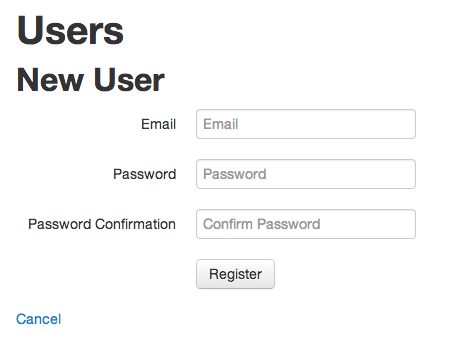
\includegraphics[width=0.5\textwidth]{images/creacion_usuario.png}
  \caption{Formulario de Creación de Usuarios}
  \label{creacion_usuario}
\end{figure}

Cuando el usuario accede de nuevo a la aplicación, esta vez en lugar de registrar un usuario debe autenticarse de modo de acceder a su información vía este pequeño formulario.

\begin{figure}[H]
  \centering
  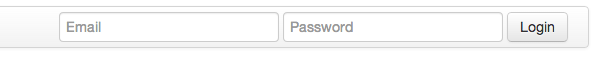
\includegraphics[width=0.5\textwidth]{images/login.png}
  \caption[Formulario de Ingreso]{\emph{Formulario de Ingreso}. Con una combinación de email y password el usuario de autentifica en el sistema.}
  \label{login}
\end{figure}

% section registro_e_ingreso_de_usuarios (end)

% ### 5.2 creación de redes sociales [screenshot]
\section{Creación de Redes Sociales} % (fold)
\label{sec:creacion_de_redes_sociales}

Dado que el usuario registró una cuenta en la aplicación, esta habilitado para crear una red social, inicialmente en la pantalla principal de redes sociales, presiona el botón \emph{Add Social Network} con el cual aparece el formulario de creación que es para darle un nombre y una descripción a la red social como detalles de esta.

\begin{figure}[H]
  \centering
  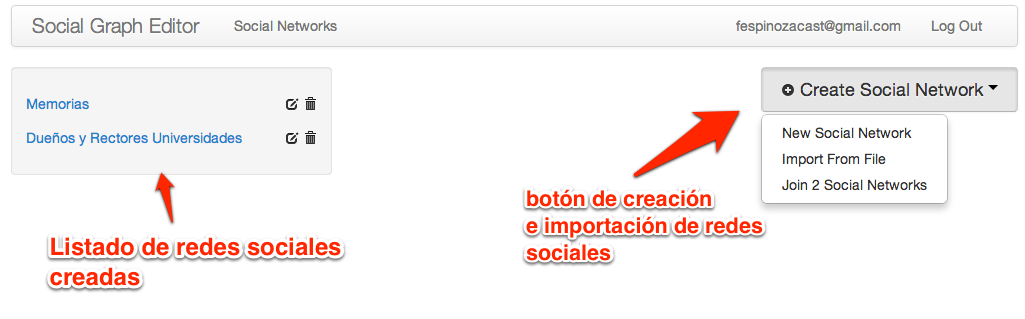
\includegraphics[width=1.0\textwidth]{images/principal_social_networks.png}
  \caption[Pantalla Principal de Redes Sociales]{\emph{Pantalla Principal de Redes Sociales}. Es la primera página luego de que el usuario se autentica, la cual le permite crear redes sociales para luego complementar su información.}
  \label{principal_social_network}
\end{figure}

\begin{figure}[H]
  \centering
  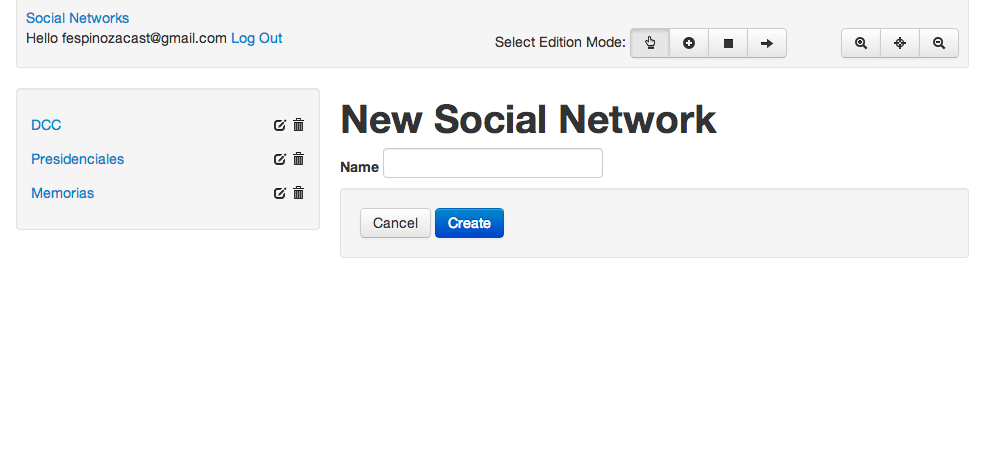
\includegraphics[width=1.0\textwidth]{images/new_social_network.png}
  \caption{Formulario Nueva Red Social}
  \label{new_social_network}
\end{figure}

Esta información ingresada de la red social, sirve como detalles de la misma y puede ser editada en cualquier momento, sin embargo, lo más relevante de la creación de la red, es la adición de contenido a la estructura de esta, lo que se cubrirá en la siguiente sección.

% section creación_de_redes_sociales (end)

\section{Edición de Redes Sociales} % (fold)
\label{sec:edicion_de_redes_sociales}

Una vez el usuario tiene su cuenta y creo una red social, este está listo para ir agregando los datos relevantes a sus redes sociales, haciendo click sobre el link con el nombre de la red social recién creada

\begin{figure}[H]
  \centering
  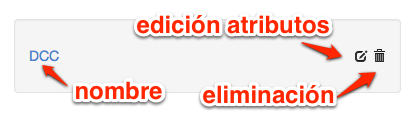
\includegraphics[width=0.5\textwidth]{images/lista_redes_sociales.png}
  \caption[Lista de Redes Sociales]{\emph{Lista de Redes Sociales}. En este lugar aparecen las redes sociales creadas, donde el nombre llega a la edición del contenido de esta, además de contar en el costado con botones para editar sus detalles o eliminar la red.}
  \label{lista_redes_sociales}
\end{figure}

\subsection{Área de Edición de Redes Sociales} % (fold)
\label{sub:area_de_edicion_de_redes_sociales}

El área de edición de redes sociales consiste básicamente de 4 elementos: el canvas donde se crea el grafo de la red social (1), una barra de herramientas para la edición (2), un área donde se definen las familias de actores y relaciones (3) y un formulario con los detalles de las entidades seleccionadas (4).

\begin{figure}[H]
  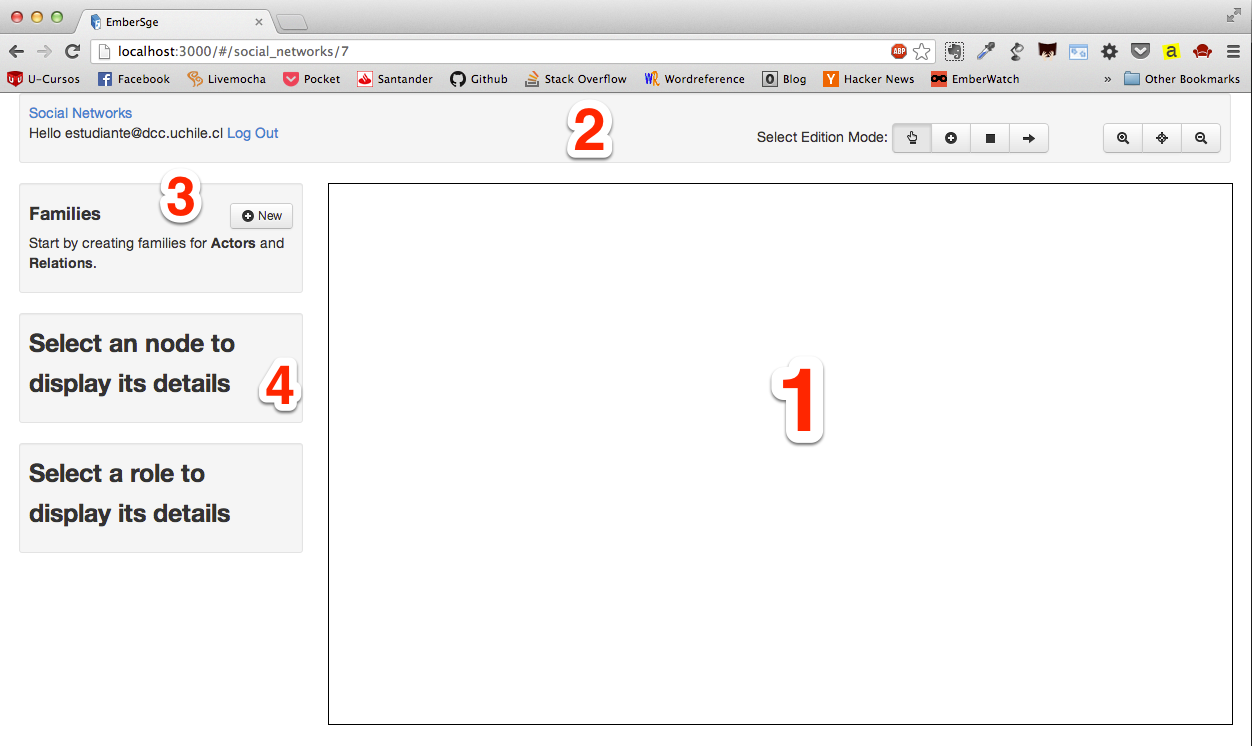
\includegraphics[width=1.0\textwidth]{images/area_edicion_redes.png}
  \caption[Área de Edición de Redes]{\emph{Área de Edición de Redes}. Esta es el área principal donde el usuario completa y manipula la información de las redes sociales creadas, con números para la explicación de las diversas secciones de esta interfaz.}
  \label{area_edicion_redes}
\end{figure}

Esta interfaz está pensada para tener la menor cantidad de elementos posibles, haciendo énfasis en las herramientas primordiales necesarias para la edición del grafo.

\subsubsection{Modos de Edición} % (fold)
\label{ssub:modos_de_edicion}

Para la zona de edición se cuenta con 4 modos de edición, de acuerdo a los cuales puedo realizar acciones diversas cuando hago click dentro de la zona del canvas.

\begin{figure}[H]
  \centering
  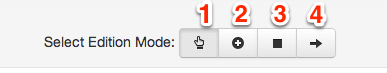
\includegraphics[width=0.5\textwidth]{images/modos_edicion.png}
  \caption[Modos de Edición]{\emph{Modos de Edición}. botones para seleccionar el modo de edición, con números para explicar los diversos modos.}
  \label{modos_edicion}
\end{figure}

Los 4 modos existentes son:

  \begin{enumerate}
    \item \textbf{Herramienta de Movimiento}: esta herramienta me permite cambiar la posición de los nodos dentro del canvas a voluntad, además de al hacer click en estos seleccionarlos para la edición de sus detalles.
    \item \textbf{Modo Actor}: en este modo, al hacer click en algún punto del canvas creará un nuevo actor dentro de esta en la posición donde se especificó haciendo click, el enfoque será puesto automáticamente en el formulario de detalles del nuevo actor para rellenar rápidamente sus campos necesarios y confirmar la creación del nuevo actor.
    \item \textbf{Modo Relación}: en este modo, al hacer click en algún punto del canvas creará una nueva relación situada en esas coordenadas, el enfoque será puesto automáticamente en el formulario de edición de la relación, pero a diferencia de los actores, las relaciones son automáticamente guardadas al momento de ser creadas y cambian al \emph{modo Rol}.
    \item \textbf{Modo Rol}: en este modo, al momento de hacer click en un actor (manteniendo el botón presionado), puedo arrastrar una flecha y situarla sobre una relación, donde al soltar el botón del mouse, creará automáticamente un nuevo rol del actor seleccionado en la relación seleccionada, para después editar sus detalles en el formulario de roles correspondiente. Además, puedo repetir esta acción cuantas veces sea necesario.
  \end{enumerate}

% subsubsection modos_de_edición (end)

% subsection área_de_edición_de_redes_sociales (end)

\subsection{Creación y Edición de Familias} % (fold)
\label{sub:creacion_y_edicion_de_familias}

Para poder agrupar los nodos (actores y relaciones) dentro de familias, hay un área reservada para la creación propia de estas familias dentro de la red, en donde a continacíon se explican las principales operaciones con familias dentro de una red social.\\

\begin{figure}[H]
  \centering
  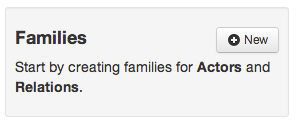
\includegraphics[width=0.6\textwidth]{images/area_familias.png}
  \caption[Área de Familias]{\emph{Área de Familias}. Detalle del área donde se crean las familias en una red social.}
  \label{area_familias}
\end{figure}

Para crear una familia se presiona el botón \emph{New} en la sección de familias, con lo que aparece un formulario con el siguiente:

\begin{figure}[H]
  \centering
  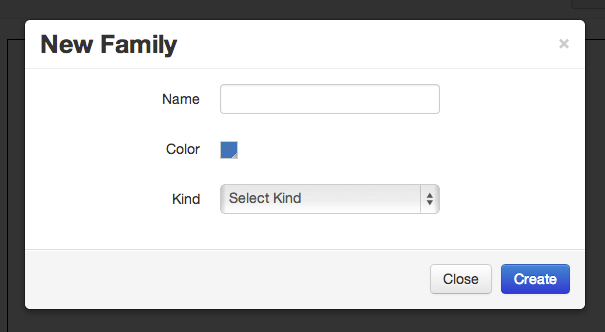
\includegraphics[width=0.7\textwidth]{images/edicion_familias.png}
  \caption[Formulario de Edición de Familias]{\emph{Formulario de Edición de Familias}. formulario por el cual se define el nombre, color y tipo de familia.}
  \label{edicion_familias}
\end{figure}

Acá se rellena el nombre y se selecciona el color para mostrar los nodos de esta familia y el tipo de nodos a los cuáles se les asignará esta familia.\\

Una vez creada, se muestra la familia en el listado con un ícono de \emph{A} para el caso de familias de actores y de \emph{R} en el caso de familias de relaciones. Donde puedo editar sus detalles o eliminarlas con los botones que se encuentran a su lado.

\begin{figure}[H]
  \centering
  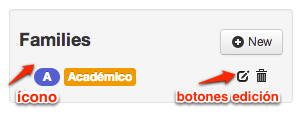
\includegraphics[width=0.5\textwidth]{images/familia_creada.png}
  \caption[Detalle Familia Creada]{\emph{Detalle Familia Creada}. un ejemplo de una familia creada, con su ícono que indica si corresponde a familia de Actores o Relaciones, además de sus botones de edición y eliminación.}
  \label{familia_creada}
\end{figure}

Es importante destacar, que se puede presionar cualquier tipo de familia, en donde al hacer esto, se cambiará al \emph{modo Actor} o \emph{modo Relación} según corresponda y a continuación cuando creo un actor o relación, por defecto pertenecerá a la familia seleccionada.

% subsection creación_y_edición_de_familias (end)

\subsection{Creación y Edición de Actores} % (fold)
\label{sub:creacion_y_edicion_de_actores}

Para crear actores, se debe definir el modo de edición a \emph{modo Actor}~\ref{ssub:modos_de_edicion}, y hacer click en el canvas donde aparecerá un actor en dicho punto y se enfocará automáticamente el formulario de creación del actor.\\

\begin{figure}[H]
  \centering
  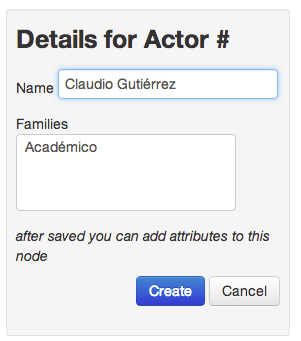
\includegraphics[width=0.5\textwidth]{images/creacion_actor.png}
  \caption{Formulario de Creación de Actor}
  \label{creacion_actor}
\end{figure}

En este formulario se puede rellenar el nombre (opcionalmente), seleccionar las familias a las que pertenece el actor para finalmente confirmar la creación, luego de esto, la información visual del actor es actualizada, mostrando al actor del color de la(s) familia(s) a la cual pertenece, además de un borde indicando de que es dicho actor el que está seleccionado en este momento.\\

\begin{figure}[H]
  \centering
  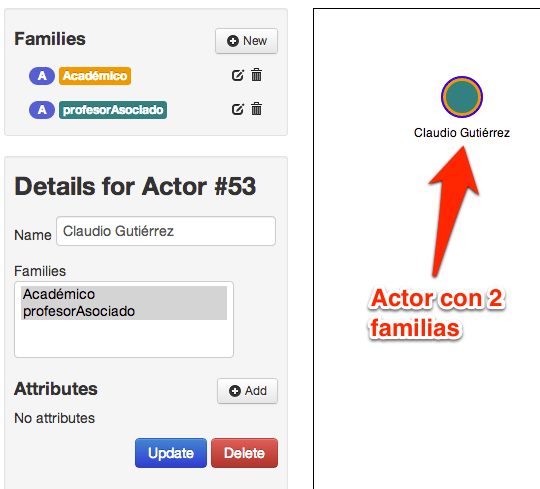
\includegraphics[width=0.6\textwidth]{images/ejemplo_actor_2_familias.png}
  \caption[Ejemplo Actor con 2 Familias]{\emph{Ejemplo Actor con 2 Familias}. Un actor con 2 familias tendrá un círculo con 2 colores de sus familias correspondientes.}
  \label{ejemplo_actor_2_familias}
\end{figure}

El actor puede ser editado en cualquier momento vía el formulario de actor, luego se presiona el botón de actualizar para persistir los cambios, o puede ser eliminado con el botón de borrar, después de confirmar en el cuadro de dialogo que aparece.

\begin{figure}[H]
  \centering
  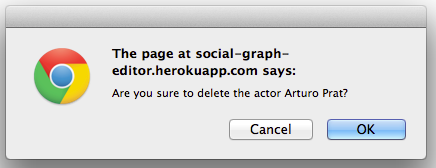
\includegraphics[width=0.5\textwidth]{images/dialogo_eliminacion_actor.png}
  \caption{Diálogo de Eliminación de Actor}
  \label{dialogo_eliminacion_actor}
\end{figure}

% subsection creación_y_edición_de_actores (end)

\subsection{Creación y Edición de Relaciones} % (fold)
\label{sub:creacion_y_edicion_de_relaciones}

Para crear una relación, se debe seleccionar el \emph{modo Relación}~\ref{ssub:modos_de_edicion}, posteriormente hacer click dentro del canvas en donde aparecerá la nueva relación y se mostrará el formulario de edición de la relación. A diferencia de los actores, las relaciones son creadas automáticamente, lo cual cambiará al modo de edición de roles, para agregar los roles correspondientes a la relación sin perder el contexto.

\begin{figure}[H]
  \centering
  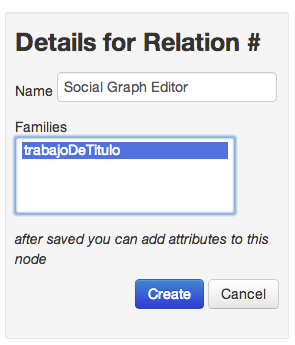
\includegraphics[width=0.5\textwidth]{images/creacion_relacion.png}
  \caption{Formulario de Creación de Relación}
  \label{creacion_relacion}
\end{figure}

% TODO check this!!! (relaciones-n-familias)
Las relaciones pueden o no tener un nombre, además de pertenecer a una familia, lo que generalmente denota el tipo de relación con la cual se está trabajando, ej: estudiaEn, dueñoDe, etc.\\

La relación puede ser editada en cualquier momento vía el formulario y presionando el botón de actualizar, o eliminada con el botón de borrar, luego de confirmar el cuadro de dialogo que aparece.

% subsection creación_y_edición_de_relaciones (end)

\subsection{Creación y Edición de Atributos en Nodos} % (fold)
\label{sub:creacion_y_edicion_de_atributos_en_nodos}

Una vez teniendo actores y relaciones creados dentro de la red social, es posible agregarles todos los atributos que se estimen conveniente por medio del formulario de edición de actores o relaciones, para esto, en la subsección de atributos en dicho formulario se puede agregar uno presionando el botón \emph{Add}, en donde puedo ingresar un atributo como un par key-value, por ejemplo puedo agregar el atributo \emph{Edad} (key) con el valor \emph{24} a un actor.

\begin{figure}[H]
  \centering
  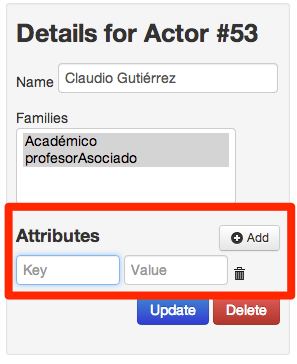
\includegraphics[width=0.5\textwidth]{images/insercion_atributos.png}
  \caption[Añadiendo Atributos a un Actor]{\emph{Añadiendo Atributos a un Actor}. se presiona el botón Add y luego se puede agregar el nuevo atributo como un par Key Value.}
  \label{insercion_atributos}
\end{figure}

Para editar atributos, se pueden editar directamente en sus campos y luego presionar el botón \emph{Update} para que los cambios sean persistidos, o borrar un atributo presionando el ícono junto a la definición del mismo.

% subsection creación_y_edición_de_atributos_en_nodos (end)

\subsection{Creación y Edición de Roles} % (fold)
\label{sub:creacion_y_edicion_de_roles}

Los roles representan la participación de un actor en una relación, dicha participación o rol, puede tener un nombre o no, un ejemplo del último caso: en una relación de amistad entre 2 personas, puede haber un tercer actor que fue quien los introdujo, pero nuevamente, el nombre de un rol es opcional. Para crear un rol, se debe seleccionar el modo de edición de roles~\ref{ssub:modos_de_edicion}, luego con el mouse, pincho un actor y arrastro el mouse hacia una relación, al soltar el mouse el rol va a ser creado inmediatamente y el foco va a ser puesto dentro del formulario de edición del rol.

\begin{figure}[H]
  \centering
  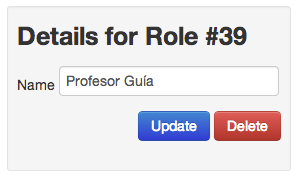
\includegraphics[width=0.5\textwidth]{images/edicion_rol.png}
  \caption[Formulario de Edición de Rol]{\emph{Formulario de Edición de Rol}. en caso de ser necesario, se puede agregar un nombre al rol o eliminarlo desde aquí.}
  \label{edicion_rol}
\end{figure}

En este formulario puedo actualizar el nombre del rol o de ser necesario eliminar el rol. Es importante mencionar que los roles sólo serán creados desde un \emph{Actor} hacia una \emph{Relación}, cualquier otra combinación no resultará en la creación de un rol.

% subsection creación_y_edición_de_roles (end)

% section edición_de_redes_sociales (end)

\section{Exportación en RDF} % (fold)
\label{sec:exportacion_en_rdf}

Como primer paso en la integración de la aplicación con la web semántica, esta permite una exportación de las redes sociales modeladas en formato N3/RDF. Con este fin, se usa la estructura de triples descrita en el modelo de mauro en la subsección~\ref{sub:representacion_como_triples}. Cabe mencionar además, que la información en la exportación comprende sólo la información de la estructura de la red social, aislándola de la información de estilos propia de la aplicación.

\begin{figure}[H]
  \centering
  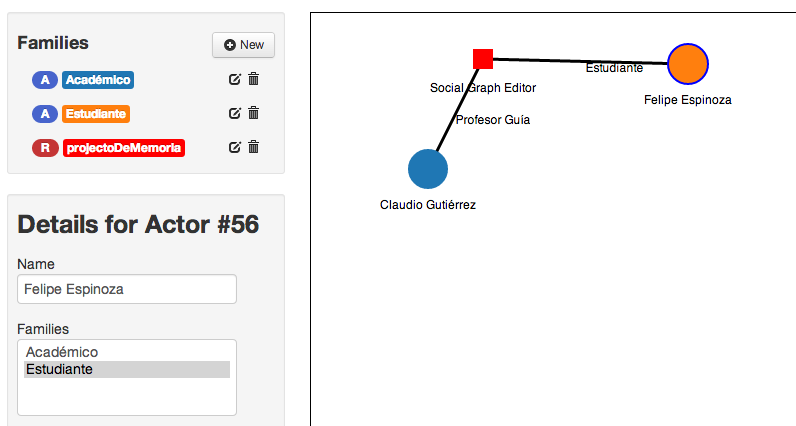
\includegraphics[width=0.8\textwidth]{images/mini_red_ejemplo.png}
  \caption[Micro Ejemplo de Red Social]{\emph{Micro Ejemplo de Red Social}. Una red social que muestra la relación de un estudiante con su profesor guía.}
  \label{mini_red_ejemplo}
\end{figure}

% TODO: mostrar como se exporta vía la interfaz y vincular eso con el resultado
A modo de ejemplo, se toma el caso de la red de la figura~\ref{mini_red_ejemplo}, que contiene 2 actores y una relación, que al exportarla en RDF quedaría de la siguiente manera.\\

\lstinputlisting[caption=Exportación RDF red social figura~\ref{mini_red_ejemplo}, style=rdf]{extra/exportacion.n3}
\label{lst:red_n3}

Es importante mencionar que dentro de dicha representación RDF se define una ontología propia de la aplicación, que cuenta con las definiciones comunes de la aplicación, como por ejemplo Actores, Relaciones y Roles, pero además cuenta con las definiciones de elementos propios de la red como Atributos definidos en esta. El vocabulario correspondiente de la red sería el siguiente:.

\lstinputlisting[caption=Vocabulario red social figura~\ref{mini_red_ejemplo}, style=rdf]{extra/vocabulary.n3}
\label{lst:vocabulario_n3}

Además, de ser necesario, se puede exportar agregando la información gráfica de la red social, en donde se incluyen las posiciones de los nodos en el canvas, los colores de las familias definidas, etc.

% section exportacion_en_rdf (end)

\section{Importación en RDF} % (fold)
\label{sec:importacion_en_rdf}

Junto con la exportación en formato RDF que usa la aplicación, esta tiene la funcionalidad de importar a partir de un archivo RDF de la red social como el definido en el ejemplo de código~\ref{lst:red_n3}, para crear una red social a partir de lo importado.

% TODO: mostrar como se importa una red social (se crea una a partir de blah blah blah)

% TODO: mencionar el algoritmo de asignación de posiciones para la red social.
Cabe destacar que el contenido N3 de la red social puede no definir las posiciones de los nodos, en caso de un archivo que fue exportado sólo con la estructura de la red, no la información visual y por lo tanto la aplicación asigna las posiciones en base al criterio \textbf{PONER CRITERIO AQUÍ}, con lo cual crea los nodos, las familias, roles e interacciones entre ellos según lo especifica el archivo usado.

% section importación_en_rdf (end)

% ### 5.6 unión de redes sociales [screenshot]
% ### 5.7 Casos de estudio
% 
% Algún ejemplo concreto de una red un poco más grande creada con esta aplicación

    \chapter{Conclusión}

\section{Evaluación de la Solución} % (fold)
\label{sec:evaluacion_de_la_solucion}

% section evaluación_de_la_solución (end)

\section{Dificultades Técnicas} % (fold)
\label{sec:dificultades_tecnicas}

% ### 6.1. Dificultades encontradas
% cosas técnicas y metodológicas que fueron complejas al momento de enfrentar la memoria

Dentro del transcurso del desarrollo de esta memoria, se encontraron algunas dificultades a nivel de implementación, razón por la cual estas serán discutidas brevemente en esta sección.

\subsection{Modelamiento de Redes Sociales} % (fold)
\label{sub:modelamiento_de_redes_sociales}

En este sentido, dentro del prototipado que requirió el abordaje del desarrollo, inicialmente se pasó por alto el modelo de Mauro San Martín \cite{tesismauro}, creando un modelo básico de redes sociales a medida que las necesidades se iban presentando en términos de desarrollo, lo cual hizo que el mismo fuera más dificultoso, lo cual forzó a estudiar de mejor manera el modelo de Mauro, que mejoró tanto la estructuración de la información, además del esfuerzo requerido para desarrollar la aplicación, ahorrando dificultades por ejemplo: de tener que manejar código para actores y relaciones separadamente en vez de considerarlos un ente común llamado nodo, entre otras cosas.\\

A continuación se presenta un listado con los puntos más relevantes con las dificultades en el modelamiento y como el modelo de Mauro ayuda con esto.

  \begin{enumerate}
    \item Considerar Actores y Relaciones como Nodos, ayuda a factorizar mucha implementación debido a que su comportamiento es casi el mismo.
    
    \item La manera de como se expresan los Roles en el modelo de Mauro permite sin mayor esfuerzo implementar una relación de $M$ a $N$ dentro de un mismo modelo (Nodo), sin mayores inconvenientes e incluso provee la convención de que un Rol posee un actor y una relación, más fácilmente implementable que especificar que sólo tuviera 2 nodos.
    
    \item El modelamiento de atributos está pensado en tener diversa clase de atributos en cantidades variables para un nodo, es decir, se puede simular la funcionalidad de una base de datos sin esquema como MongoDB con una base de datos que usa esquema como MySQL.
  \end{enumerate}


% subsection modelamiento_de_redes_sociales (end)

\subsection{Interfaz de Alta Interacción en Desarrollo Web} % (fold)
\label{sub:interfaz_de_alta_interaccion_en_desarrollo_web}

Técnicamente, si se deseaba hacer una aplicación con una alta interactividad en términos de edición de grafos y que a su vez, esta tuviera las propiedades que entrega el hecho de que sea una aplicación web, el lenguaje de programación único para completar esta tarea es JavaScript, por lo tanto, en el camino, se tuvo que adoptar un enfoque distinto al desarrollo web tradicional (\emph{server side}) y optar por el desarrollo \emph{client side}, debido a que en este se pueden acceder limpiamente todos los atributos provenientes de la base de datos, tratarlos como objetos y asignarle lógica de modelos, implementar lógicas de vista mucho más complejas que lo que se puede lograr con JavaScript plano, junto con tener mejor integración con SVG, que era necesario también para este proyecto.

Al igual que en el ítem anterior, se presenta un listado con los puntos más importantes a considerar sobre las dificultades en la elección de herramientas en el desarrollo web:

  \begin{enumerate}
    \item Una aplicación que tenga mucha interacción de interfaz, con mucha lógica en estas interacciones es mucho más fácil implementarla en un framework de desarrollo del lado del cliente como EmberJS, de acuerdo a 4 demos iniciales que usaron BackboneJS, EmberJS, Ruby on Rails con enfoques distintos para comunicar los datos del modelo al Javascript.
    
    \item Un problema de EmberJS es que para el tiempo de desarrollo, otoño 2013, ember-data, el proyecto que comunica el \emph{back-end} de la aplicación con su \emph{front-end} en EmberJS, es bastante inestable, sin embargo, posee una comunidad activa que actualiza las versiones de este proyecto rápidamente.
    
    \item Para representar los elementos manipulables en el Canvas de Redes Sociales, la mejor opción fue usar D3.js para generar los gráficos vectoriales, que son tags dentro del documento HTML, por lo cual, es más simple asignarles eventos para poder interactuar con esos elementos. Además D3.js puede obtener y usar los datos de la misma forma que EmberJS los provee, por lo tanto la integración es más fácil.
  \end{enumerate}

% subsection interfaz_de_alta_interacción_en_desarrollo_web (end)


% section dificultades_técnicas (end)

\section{Trabajo Futuro} % (fold)
\label{sec:trabajo_futuro}

A partir de lo realizado, se pueden encontrar los siguientes pasos a futuro con este proyecto:

  \begin{enumerate}
    \item \textbf{Agregar Endpoint SPARQL}: uno de los aspectos técnicos a futuro, sería la instalación de un endpoint virtuoso, u otro para aprovechar de mejor manera la utilización del formato RDF, de esta forma, reemplazar el almacenamiento relacional de los datos por uno de grafos y lograr una mayor integración con la web semántica.
    
    \item \textbf{Mejorar Escalabilidad Aplicación}: Si el proyecto llega a un nivel popularidad grande, se puede mejorar la escalabilidad de manera tal de que la aplicación soporte redes sociales de mayor tamaño, sin perder performance de la misma.
    
    \item \textbf{Habilitar Modo Offline Aplicación}: Es posible, debido a la utilización de frameworks client side, hacer que la aplicación de edición de grafos me permita un modo offline, reemplazando el almacenamiento centralizado por uno local en el navegador, sincronizando los datos si es pertinente posteriormente.
    
    \item \textbf{Temporalidad en Redes Sociales}: se puede extender la aplicación de manera tal de que se pueda agregar temporalidad a las redes sociales, que sirva para analizar los cambios en las estructuras sociales con el paso del tiempo, aspecto que puede ser prometedor para la utilidad de esta herramienta en el estudio de ciertas disciplinas relacionadas con redes sociales.
    
    \item \textbf{Aspectos de Privacidad}: la aplicación se puede mejorar en términos de privacidad de los datos, explicitando que los datos agregados a la aplicación son de propiedad exclusiva de sus usuarios, que no habrá ningún tipo de mal uso de la información, además de agregar opciones para diferenciar redes privadas y públicas con sus restricciones de permisos peritnentes.
    
    \item \textbf{Aspectos Legales}: Se debe resolver además temas legales con respecto a la aplicación y la publicación de datos privados de personas, en redes sociales de tipo público, que pudieran legalmente afectar de una u otra forma a terceros por la exposición de estos datos.
  \end{enumerate}

% section trabajo_futuro (end)
  %=== END cuerpo memoria
  
  \nocite{*}
  \bibliographystyle{plain}
  \bibliography{endings/02-bibliography}
\end{document}